\documentclass[10pt,twocolumn,letterpaper]{article}
\usepackage[margin=0.68in,top=0.72in,bottom=0.72in]{geometry}
\usepackage{graphicx,amsmath,booktabs,microtype,url}
\setlength{\columnsep}{0.22in}
\title{Bagging, Boosting and Bias--Variance on Face Recognition}
\author{Abhishek Kapar\\Roll No. M26ecm511\\Repository: \url{https://github.com/m26ecm511-cpu/ML-Assignment-2-Bagging-Boosting}}\date{}
\begin{document}\maketitle
\begin{abstract}
We compare a decision-tree baseline, bootstrap aggregation, and multiclass SAMME boosting on the Olivetti Faces dataset using raw 4096-dimensional pixel vectors. A fixed identity-wise split was used for training, validation, and clean testing. Robustness was evaluated by zeroing a central 16 by 16 image block. Empirical squared bias and variance were measured over 30 identity-wise bootstrap refits. All numerical results below are generated by the accompanying reproducible code.
\end{abstract}
\section{Experimental protocol}
The dataset has 40 identities, ten 64 by 64 images per identity, and 4096 raw pixel features per image. The seed is 26511, derived from the numeric characters in the roll number. Each identity contributes six training, two validation, and two clean test images, giving 240/80/80 examples. The split is saved in \texttt{outputs/split.json} and reused. No PCA or dimensionality reduction is applied. For robustness, rows 24--39 and columns 24--39 are set to zero in a copy of the test images; training remains clean.
\section{Decision tree and bagging}
We selected the tree configuration using validation accuracy over maximum depths 2, 4, 8, 16 and unlimited, and minimum leaf sizes 1, 2 and 4. The selected depth was None and minimum leaf size was 4. It achieved training, validation and clean-test accuracy of 0.975, 0.575 and 0.625.
Bagging was implemented directly by drawing bootstrap samples and taking majority votes. Table~\ref{tab:main} reports the final models. The ensemble-size sweep is shown in Table~\ref{tab:bag}. For a bootstrap sample of size n, the expected number of distinct training examples is $n[1-(1-1/n)^n]$, approximately $0.632n$. The expected omitted fraction is approximately $e^{-1}=0.368$. The empirical distinct counts and OOB diagnostics are recorded in the JSON output.
Pairwise disagreement measures the fraction of test examples on which two trees differ. Vote margin is the winning vote fraction minus the runner-up fraction. These diagnostics characterize ensemble diversity and decisiveness; neither guarantees correctness.
\begin{table}[t]\centering\scriptsize
\caption{Bagging ensemble-size sweep. Distinct examples is averaged per bootstrap sample.}\label{tab:bag}
\begin{tabular}{rrrrrr}\toprule
$B$ & Train & Val. & Test & OOB & Distinct\\\midrule
1 & 0.708 & 0.325 & 0.487 & 0.350 & 160.000 \\
5 & 0.963 & 0.537 & 0.625 & 0.373 & 154.200 \\
10 & 0.988 & 0.662 & 0.800 & 0.432 & 155.600 \\
25 & 1.000 & 0.812 & 0.875 & 0.592 & 154.000 \\
50 & 1.000 & 0.863 & 0.900 & 0.704 & 153.220 \\
100 & 1.000 & 0.875 & 0.925 & 0.738 & 152.370 \\
200 & 1.000 & 0.850 & 0.950 & 0.792 & 152.115 \\
\bottomrule\end{tabular}\end{table}
\section{Multiclass SAMME boosting}
For K classes and weighted error $\epsilon_t$, SAMME uses $\alpha_t=\log((1-\epsilon_t)/\epsilon_t)+\log(K-1)$. Sample weights are multiplied by $\exp(\alpha_t I[h_t(x_i)\ne y_i])$ and normalized. Learners with error no better than random multiclass prediction are rejected. The selected model used maximum tree depth 4
 and 100 requested rounds, selected by validation accuracy only. Table~\ref{tab:boostcompare} compares the required 25, 50 and 100 learner runs. Round-wise weighted error, learner weight, maximum sample weight and top-ten weight mass are included in the accompanying figures and JSON files. Bagging reduces variance through averaging; boosting sequentially emphasizes examples misclassified by prior learners.
\begin{table}[t]\centering\scriptsize
\caption{SAMME learner-count comparison at selected depth.}\label{tab:boostcompare}
\begin{tabular}{rrrrr}\toprule
Rounds (used) & Train & Val. & Test & Seconds\\\midrule
25 (25) & 0.537 & 0.200 & 0.287 & 26.081 \\
50 (50) & 0.733 & 0.300 & 0.362 & 52.887 \\
100 (100) & 1.000 & 0.338 & 0.512 & 104.537 \\
\bottomrule\end{tabular}\end{table}
\section{Clean and masked test performance}
Table~\ref{tab:main} compares clean and masked accuracy, empirical squared bias and variance. The confidence measure for bagging is its normalized vote fraction. For SAMME, normalized class scores are weighted vote fractions, not calibrated probabilities. Masking removes information from every test image, so ensemble averaging cannot recover the missing pixels; the measured difference between clean and masked accuracy quantifies the effect for each model.
\begin{table}[t]\centering\small
\caption{Measured clean/masked accuracy and empirical bias--variance.}\label{tab:main}
\begin{tabular}{lrrrr}\toprule
Model & Clean & Masked & Bias$^2$ & Variance\\\midrule
Single tree & 0.625 & 0.287 & 0.308 & 0.579 \\
Bagging & 0.925 & 0.800 & 0.480 & 0.025 \\
SAMME boosting & 0.512 & 0.362 & 0.876 & 0.017 \\
\bottomrule\end{tabular}\end{table}
\section{Bias--variance experiment}
We kept the clean test set fixed and created 30 resampled training sets, sampling six training images with replacement within each identity. No hyperparameter tuning was repeated. With $p_r(x_i)$ denoting the class vector for refit r, $\bar p(x_i)$ its average, and $e_i$ the one-hot target, we computed $N^{-1}\sum_i\|\bar p(x_i)-e_i\|_2^2$ and $(NR)^{-1}\sum_{i,r}\|p_r(x_i)-\bar p(x_i)\|_2^2$. Test accuracy mean and standard deviation are provided in the results JSON. The depth comparison is summarized in Table~\ref{tab:depth}. The deepest tree need not yield the largest bagging improvement: the observed result depends on leaf occupancy, bias, variance and disagreement.
\begin{table}[t]\centering\scriptsize
\caption{Depth study: single trees and 100-tree bagging ensembles.}\label{tab:depth}
\begin{tabular}{rrrrr}\toprule
Depth & Tree accuracy & Leaves & Bag accuracy & Disagreement\\\midrule
2 & 0.0633 & 3.07 & 0.1517 & 0.9604 \\
4 & 0.0967 & 5.10 & 0.3017 & 0.9473 \\
8 & 0.1646 & 9.33 & 0.5108 & 0.9254 \\
16 & 0.2833 & 17.60 & 0.7154 & 0.8837 \\
\bottomrule\end{tabular}\end{table}
\begin{figure}[t]\centering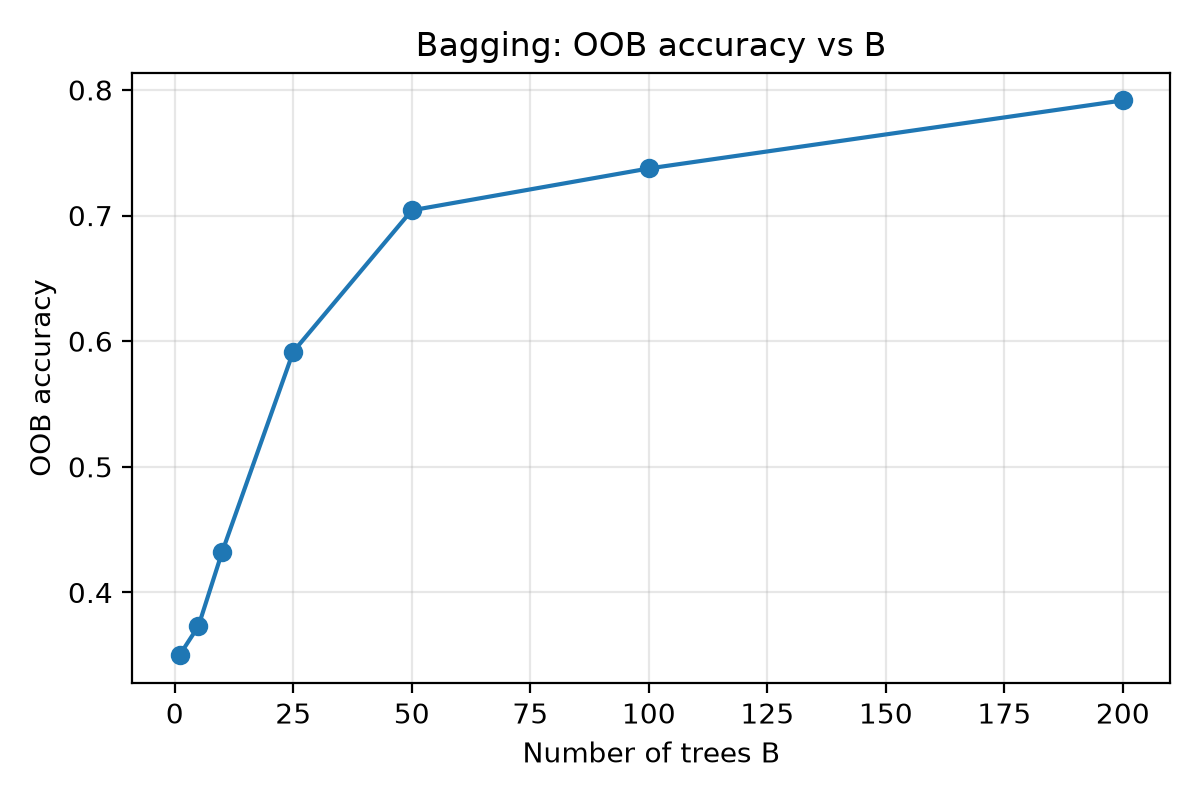
\includegraphics[width=\linewidth]{figures/q1_oob_accuracy.png}\caption{OOB accuracy as a function of ensemble size.}\end{figure}
\begin{figure}[t]\centering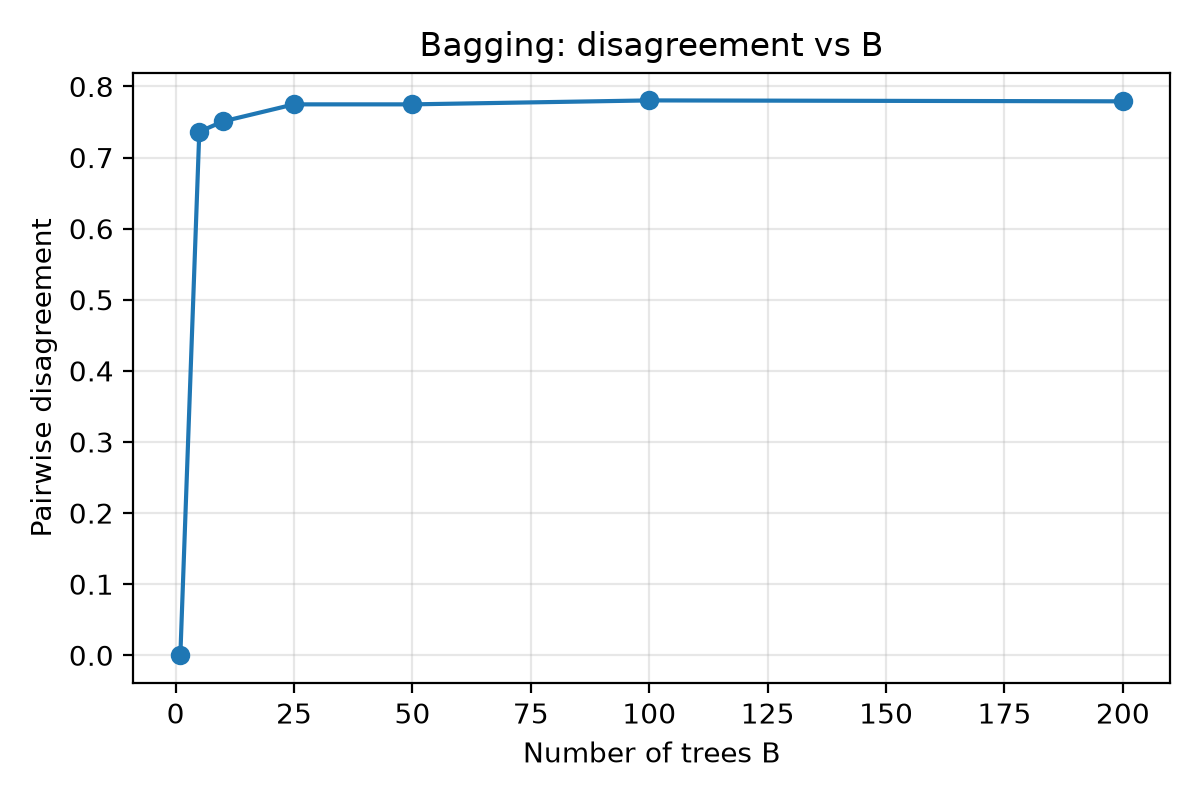
\includegraphics[width=\linewidth]{figures/q1_disagreement.png}\caption{Mean pairwise tree disagreement.}\end{figure}
\begin{figure}[t]\centering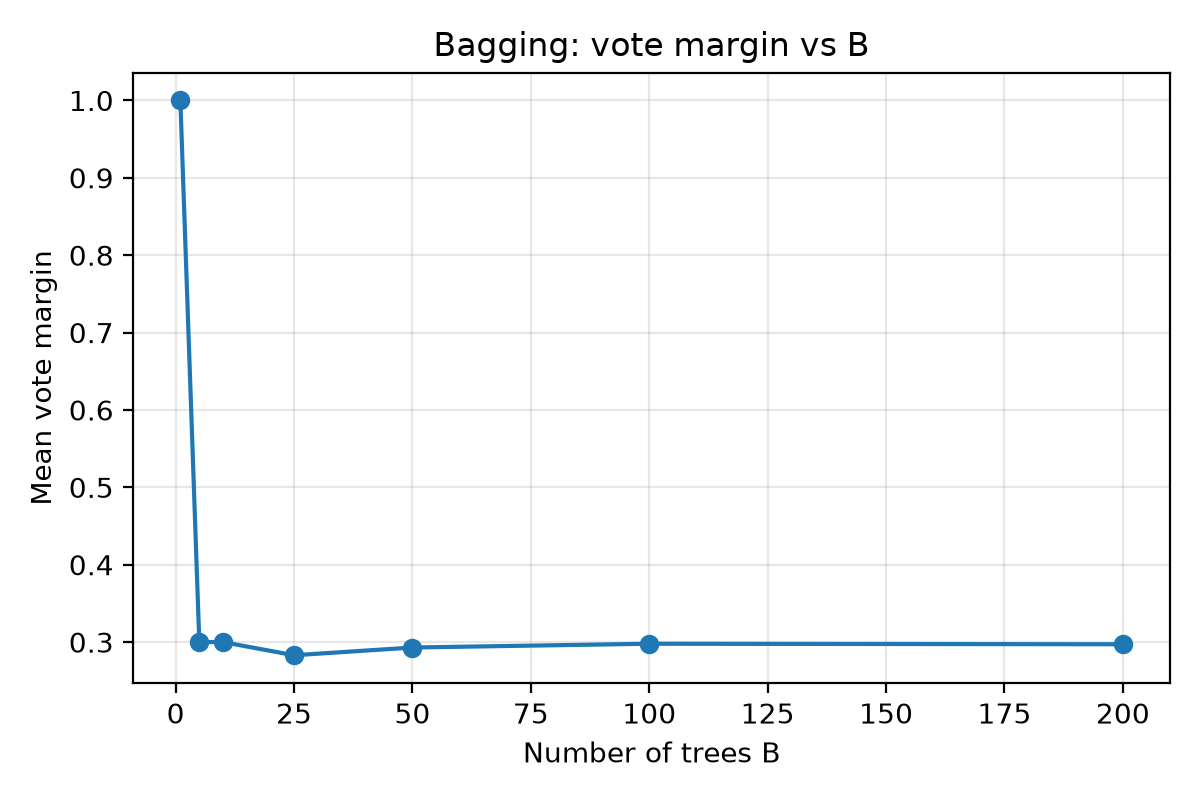
\includegraphics[width=\linewidth]{figures/q1_vote_margin.png}\caption{Mean bagging vote margin.}\end{figure}
\begin{figure}[t]\centering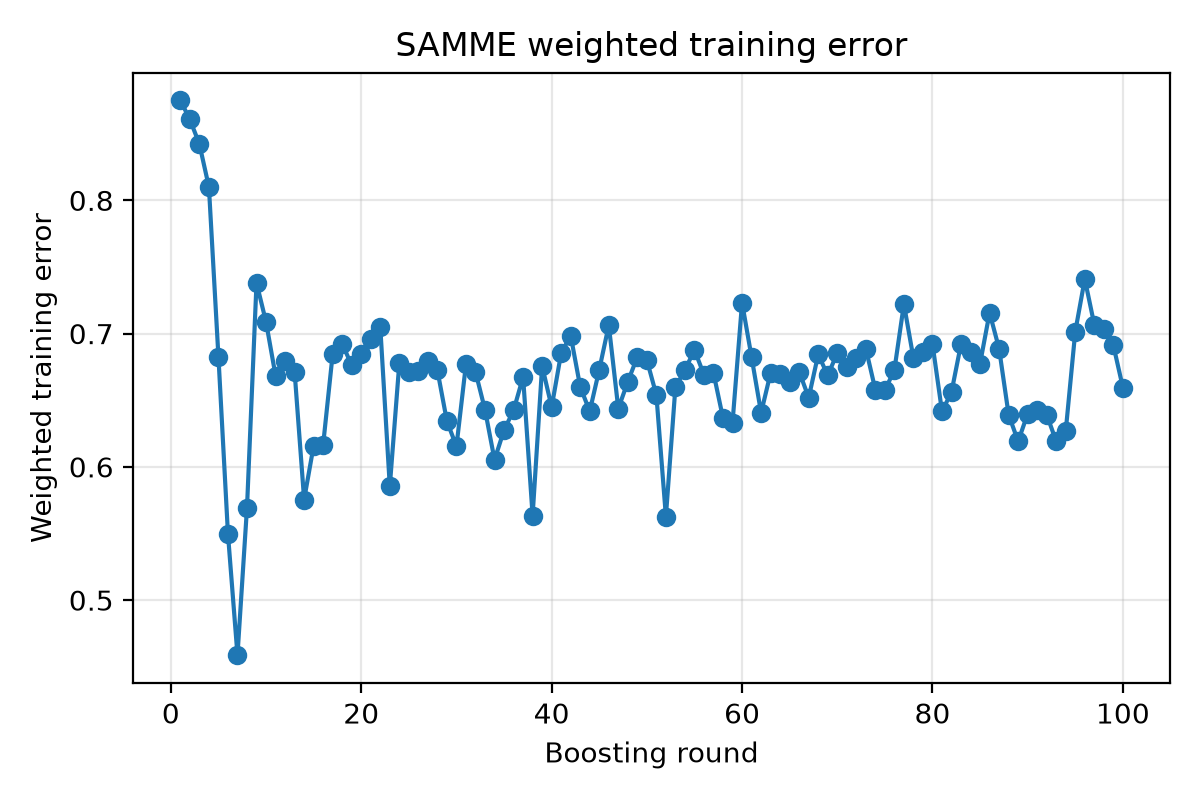
\includegraphics[width=\linewidth]{figures/q2_weighted_training_error.png}\caption{SAMME weighted training error.}\end{figure}
\begin{figure}[t]\centering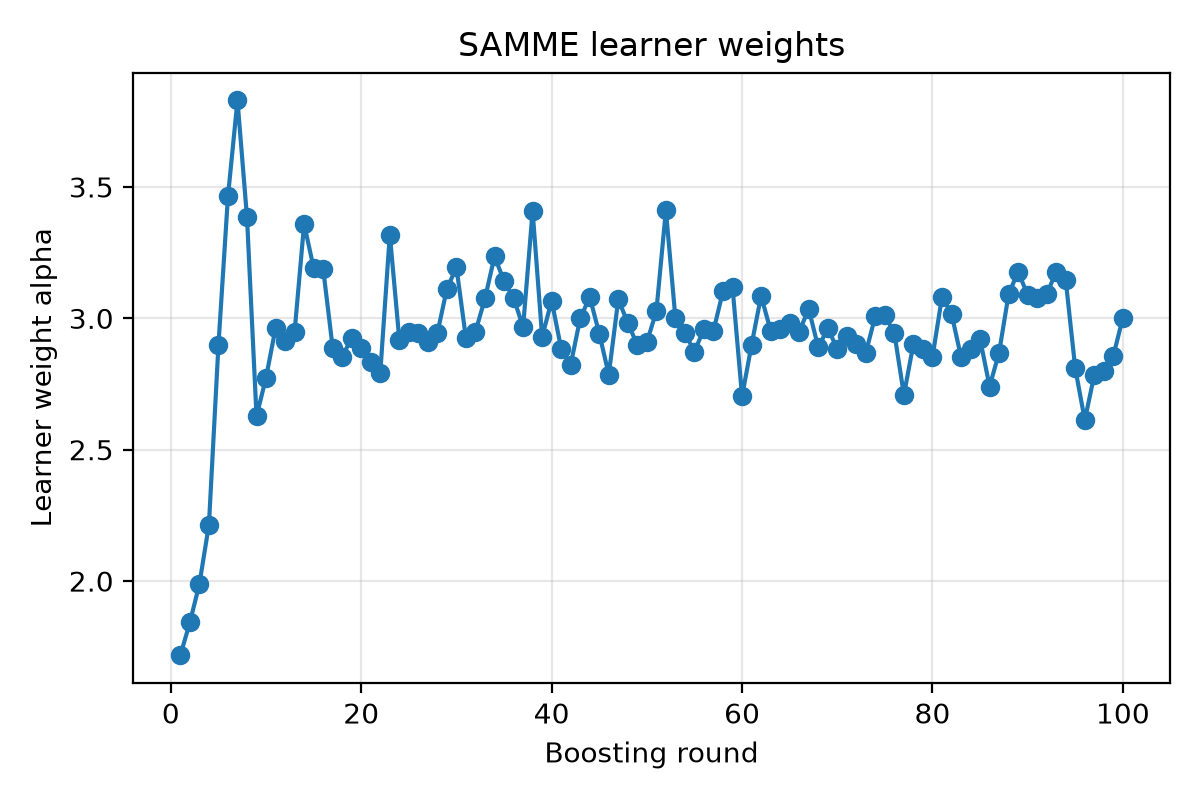
\includegraphics[width=\linewidth]{figures/q2_learner_weights.png}\caption{SAMME learner weights.}\end{figure}
\begin{figure}[t]\centering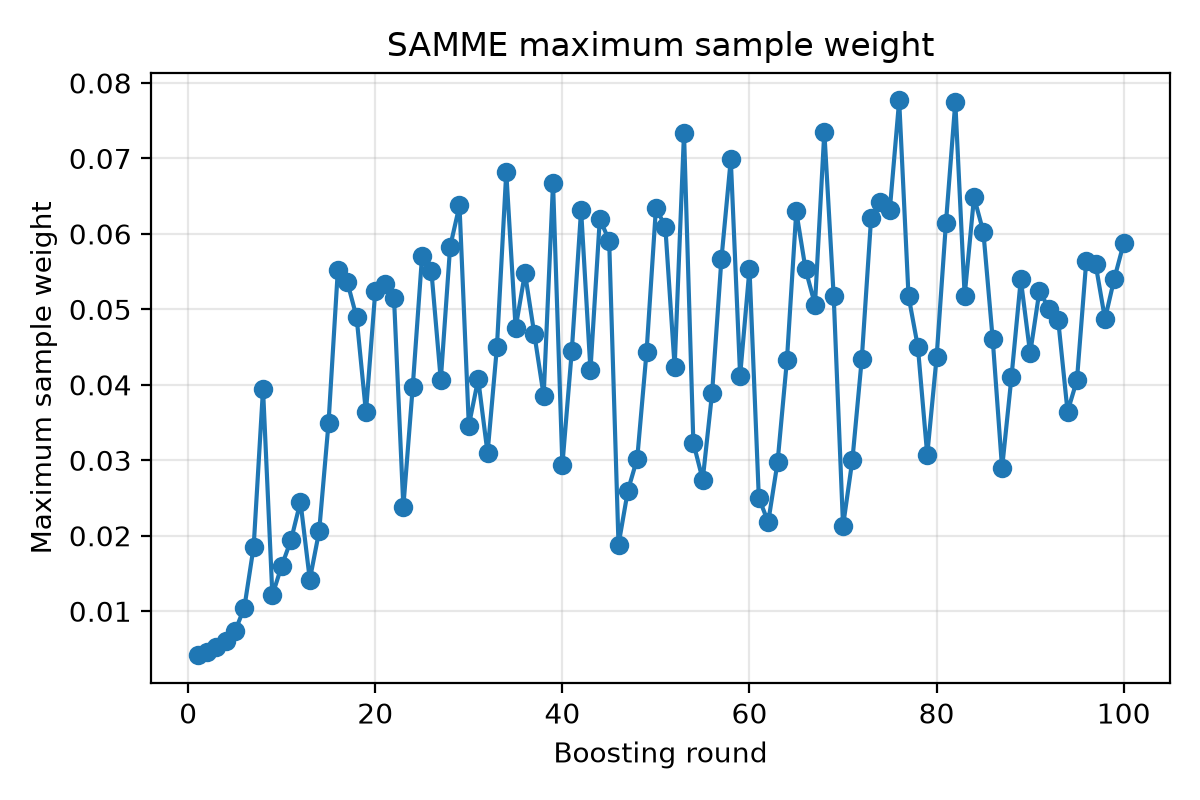
\includegraphics[width=\linewidth]{figures/q2_max_sample_weight.png}\caption{Maximum sample weight by round.}\end{figure}
\begin{figure}[t]\centering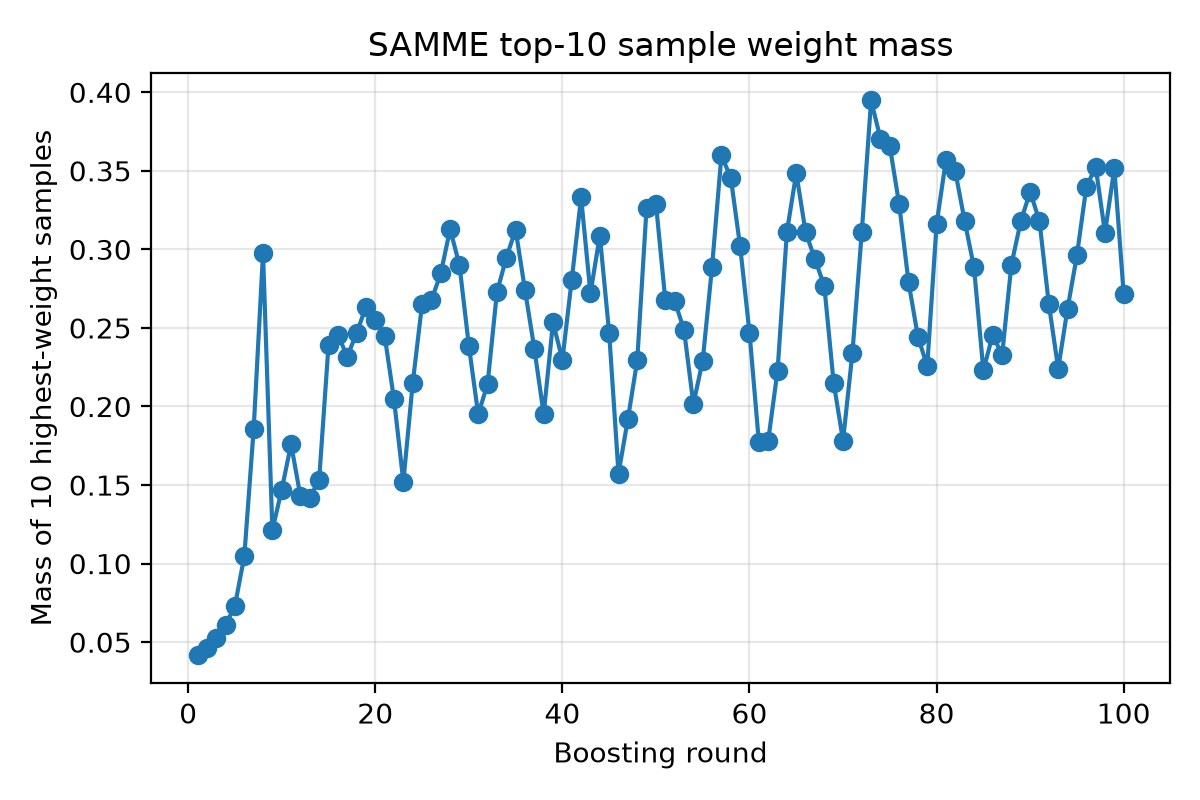
\includegraphics[width=\linewidth]{figures/q2_top10_weight_mass.png}\caption{Weight mass of the ten highest-weight samples.}\end{figure}
\begin{figure}[t]\centering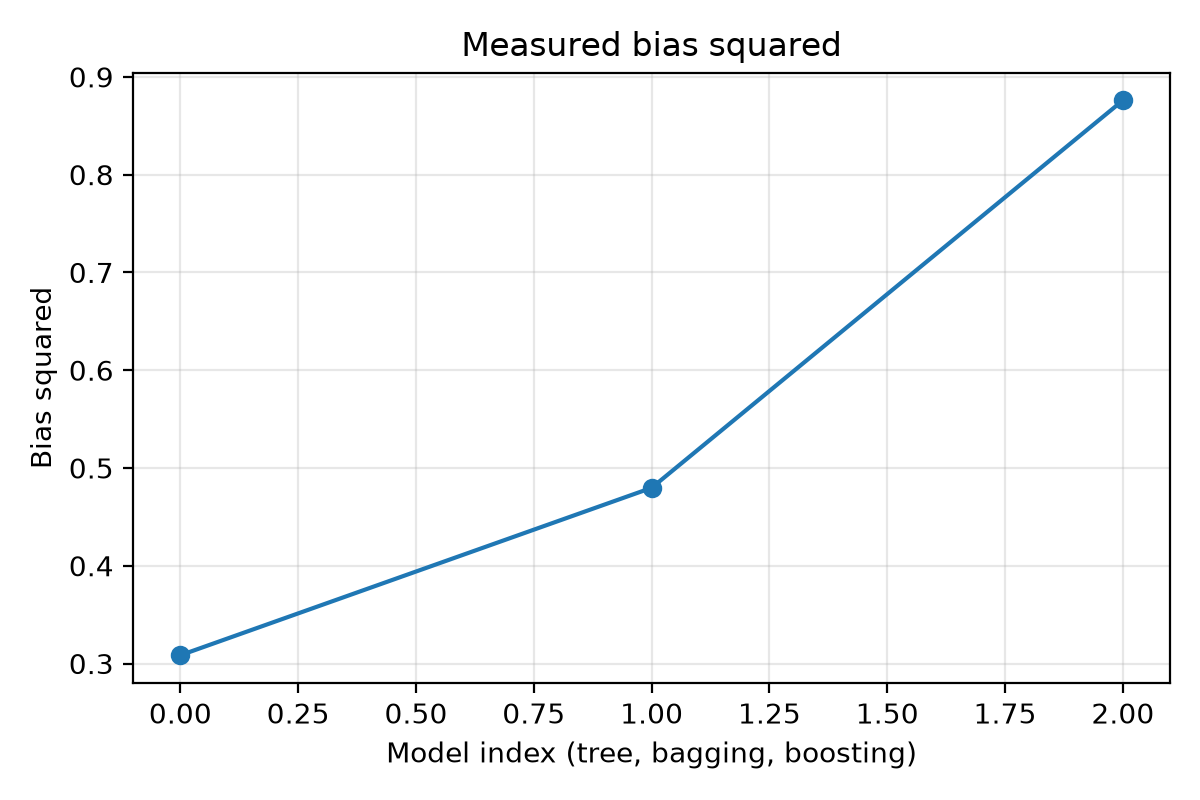
\includegraphics[width=\linewidth]{figures/q3_bias_squared.png}\caption{Empirical squared bias by model.}\end{figure}
\begin{figure}[t]\centering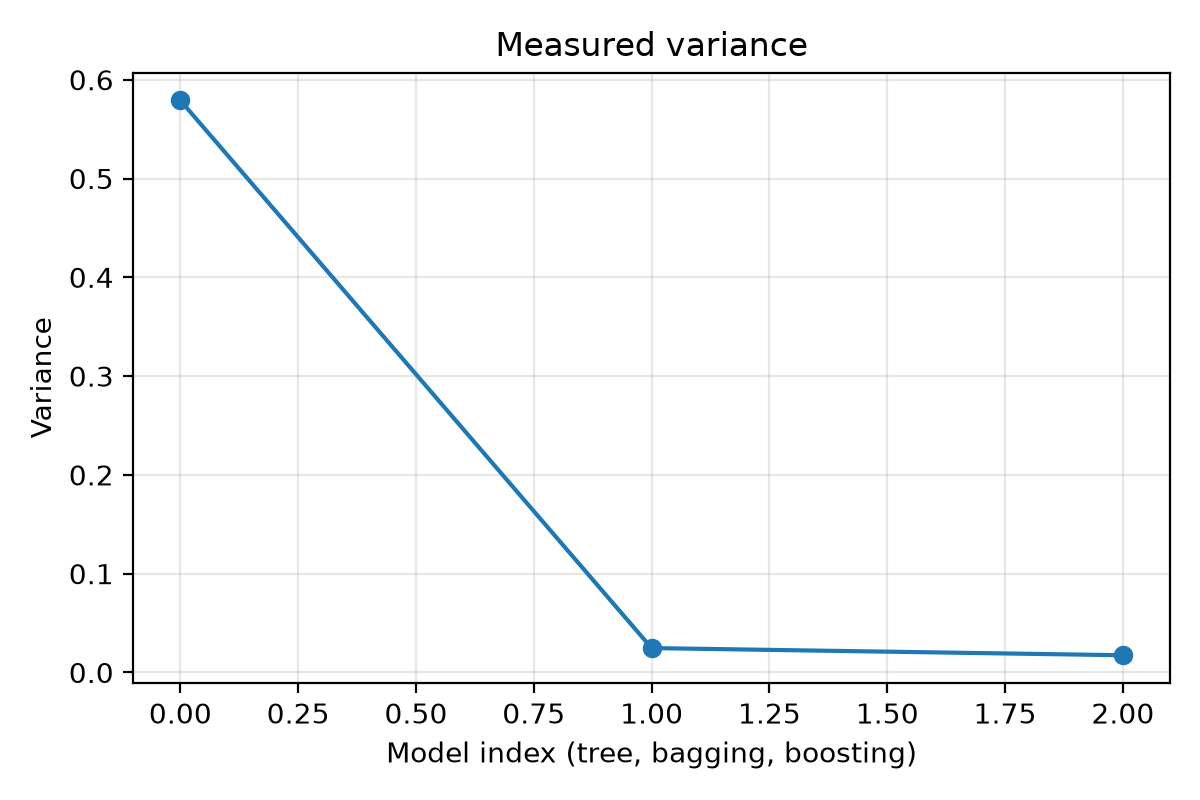
\includegraphics[width=\linewidth]{figures/q3_variance.png}\caption{Empirical variance by model.}\end{figure}
\section{Conclusion}
The measured results indicate that the most stable model is bagging, the model most sensitive to the missing region is single\_tree, and the highest clean-test accuracy is bagging. These labels should be interpreted alongside the reported metrics rather than as universal properties of the algorithms.
\section*{References}
\noindent [1] AT\&T Laboratories Cambridge, Olivetti Faces dataset, 1992--1994.

\noindent [2] F. Pedregosa et al., ``Scikit-learn: Machine Learning in Python,'' \emph{JMLR}, vol. 12, pp. 2825--2830, 2011.

\noindent [3] Y. Freund and R. E. Schapire, ``A Decision-Theoretic Generalization of On-Line Learning and an Application to Boosting,'' \emph{JCSS}, 1997.\end{document}
